\documentclass[text01.tex]{subfiles}
\begin{document}
%
% Chapter 1
% 
\chapter{ラズベリーパイの使い方・\\自己紹介ページを作ろう}

% 
% section 1.1
% 
\section{今回の授業}

% 
% subsection 1.1.1
% 
\subsection{目標と\ruby{授業内容}{じゅぎょうないよう}}

% 
% subsubsection 1
% 
\subsubsection{目標}

\begin{itemize}
  \item ラズベリーパイになれよう
  \item 自分のホームページを作れるようになろう
\end{itemize}

% 
% subsubsection 2
% 
\subsubsection{\ruby{授業内容}{じゅぎょうないよう}}

\begin{enumerate}
  \item ラズベリーパイとは
  \item ラズベリーパイになれよう（１）
  \item ラズベリーパイになれよう（２）
  \item 自分の\ruby{紹介}{しょうかい}ページを作ろう
\end{enumerate}

% 
% subsubsection 3
% 
\subsubsection{注意点}

\begin{itemize}
  \item \ruby{授業}{じゅぎょう}の合間のきゅうけいでは、遠くのものをながめたりして目を休めましょう
  \item 水分\ruby{補給}{ほきゅう}はこまめにしましょう
  \item 先生が説明中は先生の話を聞きましょう
  \item わからないことがあったらTAの先生方にすぐ聞きましょう
\end{itemize}

% 
% subsubsection 4
% 
\subsubsection{教科書について}

教科書では、\ruby{具体的}{ぐたいてき}な操作の手順が説明され、それを\ruby{応用}{おうよう}した問題があります。
まずは、説明をよく読みながら試してみましょう。
そのあと問題を\ruby{解}{と}きましょう。
% 問題の答えは一番最後のページにあります。
% \clearpage

% 
% subsubsection 5
% 
\subsubsection{\ruby{配布物}{はいふぶつ}の\ruby{確認}{かくにん}}

\begin{minipage}[b]{0.45\linewidth}
  \begin{enumerate}
    \item ラズベリーパイ
    \item SDカード
    \item \ruby{電源}{でんげん}ケーブル
    \item HDMIケーブル
    \item GPIOエクステンダー
  \end{enumerate}  
\end{minipage}
%
\begin{minipage}[b]{0.45\linewidth}
  \begin{enumerate}
    \setcounter{enumi}{5}
    \item ヘッドセット
    \item マウス
    \item センサーボード
    \item ウェブカメラ
    \item ディスプレイ(持って帰れません)
  \end{enumerate}
\end{minipage}
\bigskip

\begin{figure}[htbp]
  \begin{minipage}[b]{0.3\linewidth}
    \centering
    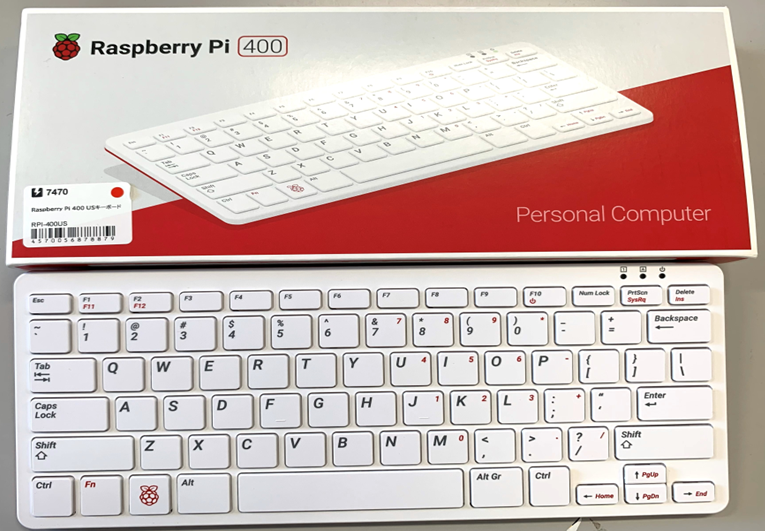
\includegraphics[keepaspectratio, height=30mm]{../../asset/image/fig_001_01_2025.png}
    \newline
    \small{1. ラズベリーパイ}
    \newline
  \end{minipage}
  %
  \begin{minipage}[b]{0.3\linewidth}
    \centering
    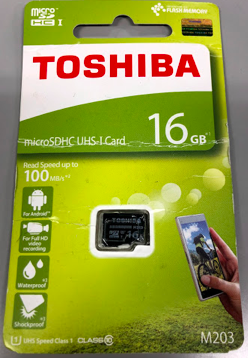
\includegraphics[keepaspectratio, height=30mm]{../../asset/image/fig_001_02_2025.png}
    \newline
    \small{2. SDカード}
    \newline
  \end{minipage}
  %
  \begin{minipage}[b]{0.3\linewidth}
    \centering
    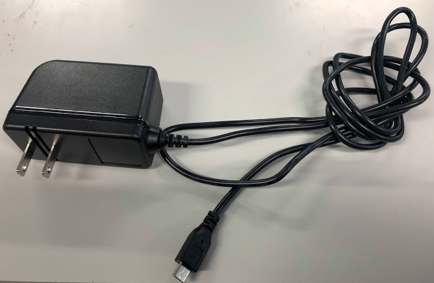
\includegraphics[keepaspectratio, height=30mm]{../../asset/image/fig_001_03_2025.png}
    \newline
    \small{3. 電源ケーブル}
    \newline
  \end{minipage}
  %
  %
  \begin{minipage}[b]{0.3\linewidth}
    \centering
    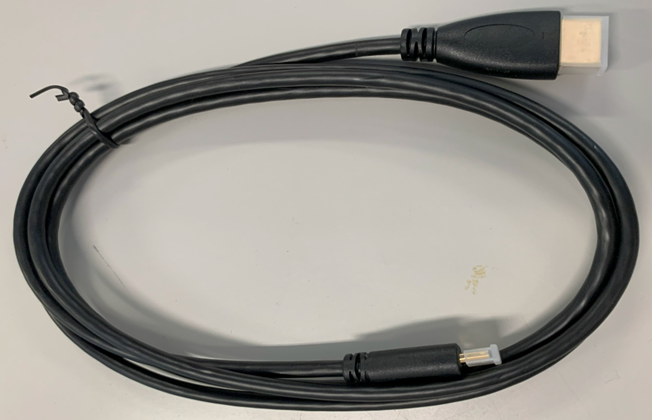
\includegraphics[keepaspectratio, width=45mm]{../../asset/image/fig_001_04_2025.png}
    \newline
    \small{4. HDMIケーブル}
    \newline
  \end{minipage}
  %
  \begin{minipage}[b]{0.3\linewidth}
    \centering
    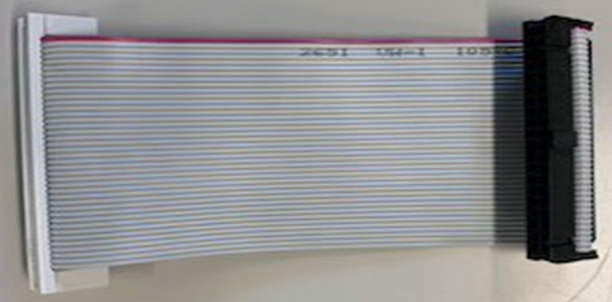
\includegraphics[keepaspectratio, width=45mm]{../../asset/image/fig_001_05_2025.png}
    \newline
    \small{5. GPIOエクステンダー}
    \newline
  \end{minipage}
  %
  \begin{minipage}[b]{0.3\linewidth}
    \centering
    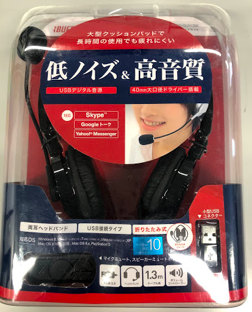
\includegraphics[keepaspectratio, height=30mm]{../../asset/image/fig_001_06_2025.png}
    \newline
    \small{6. ヘッドセット}
    \newline
  \end{minipage}
  %
  %
  \begin{minipage}[b]{0.3\linewidth}
    \centering
    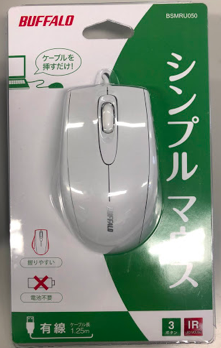
\includegraphics[keepaspectratio, height=30mm]{../../asset/image/fig_001_07_2025.png}
    \newline
    \small{7. マウス}
    \newline
  \end{minipage}
  %
  \begin{minipage}[b]{0.3\linewidth}
    \centering
    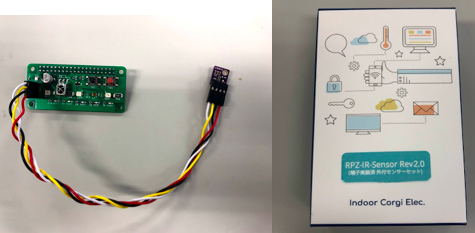
\includegraphics[keepaspectratio, width=45mm]{../../asset/image/fig_001_08_2025.png}
    \newline
    \small{8. センサーボード}
    \newline
  \end{minipage}
  %
  \begin{minipage}[b]{0.3\linewidth}
    \centering
    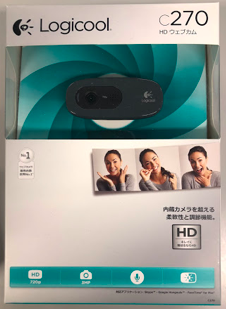
\includegraphics[keepaspectratio, height=30mm]{../../asset/image/fig_001_09_2025.png}
    \newline
    \small{9. ウェブカメラ}
    \newline
  \end{minipage}
  %
  %
  \begin{minipage}[b]{0.3\linewidth}
    \centering
    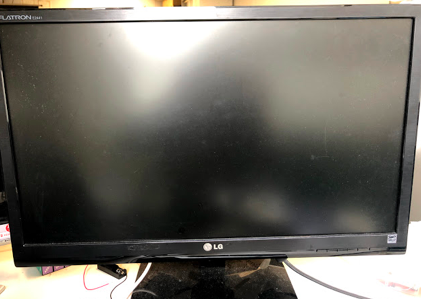
\includegraphics[keepaspectratio, width=45mm]{../../asset/image/fig_001_10_2025.png}
    \newline
    \small{10. ディスプレイ}
    \newline
  \end{minipage}
\end{figure}
\newpage


% 
% subsection 1.1.2
% 
\subsection{ラズベリーパイについて}

イギリスのラズベリーパイ\ruby{財団}{ざいだん}が開発したコンピュータです。
いろいろな\ruby{種類}{しゅるい}がありますが、子どもIT\ruby{未来塾}{みらいじゅく}では
キーボード一体型のタイプを使用しています。
ラズベリーパイはラズパイとも\ruby{呼}{よ}ばれています。

% 
% subsubsection 1
% 
\subsubsection{\ruby{特徴}{とくちょう}}

\begin{itemize}
  \item キーボード一体型で、キーボードが必要ない
  \item \ruby{普通}{ふつう}のパソコンのように使える(動画\ruby{再生}{さいせい}やゲームもできます)
  \item プログラミングの\ruby{勉強}{べんきょう}に向いている
  \item モータやライトを\ruby{制御}{せいぎょ}できる(目に見えるのでプログラミングを楽しめる)
\end{itemize}

% 
% subsubsection 2
% 
\subsubsection{ラズベリーパイでできること}

プログラミングを手軽に学ぶことができます。
プログラミングするにはパソコンが必要でお金もかかるため、やりたくてもできない人も
いたかもしれません。
しかし、ラズベリーパイのような小さくて手に入れやすいコンピュータがあれば手軽に
プログラミングの学習に取り組むことができます。
また、ラズベリーパイを使うことでモータを動かしたりライトを光らせたりすることができます。
これらの\ruby{制御}{せいぎょ}をプログラムで実行できるため、楽しみながら学習を進められます。

% 
% subsubsection 3
% 
\subsubsection{ラズベリーパイを使うときの注意}

\begin{itemize}
  \item 水などぬれているものをラズベリーパイ本体につけないようにしましょう
  \item ラズベリーパイ（コンピュータなど）は熱に弱いのですごく暑い部屋では使わないようにしましょう
  \item ラズベリーパイなどは静電気に弱いので注意しましょう
  \item ラズベリーパイをらんぼうに\ruby{扱}{あつか}うのはやめましょう
\end{itemize}
\clearpage

% 
% subsection 1.1.10
% 
\subsection{パスワードについて学ぼう}

% 
% subsubsection
% 
\subsubsection{パスワードの\ruby{重要性}{じゅうようせい}について知ろう}
\vspace*{5mm}

IDとパスワードは、タブレットやパソコンなどの\ruby{情報機器}{じょうほうきき}や、
インターネット上のサービスを利用する\ruby{際}{さい}に、\ruby{許可}{きょか}された者であるかを
\ruby{識別}{しきべつ}し、本人を\ruby{確認}{かくにん}するための重要な\ruby{情報}{じょうほう}です。
いわゆるインターネットやパソコンなどの電子機器に入るための\ruby{鍵}{かぎ}の名前（ユーザーID）と
その\ruby{鍵}{かぎ}（パスワード）のようなものです。
%
\begin{figure}[h]
  \centering
  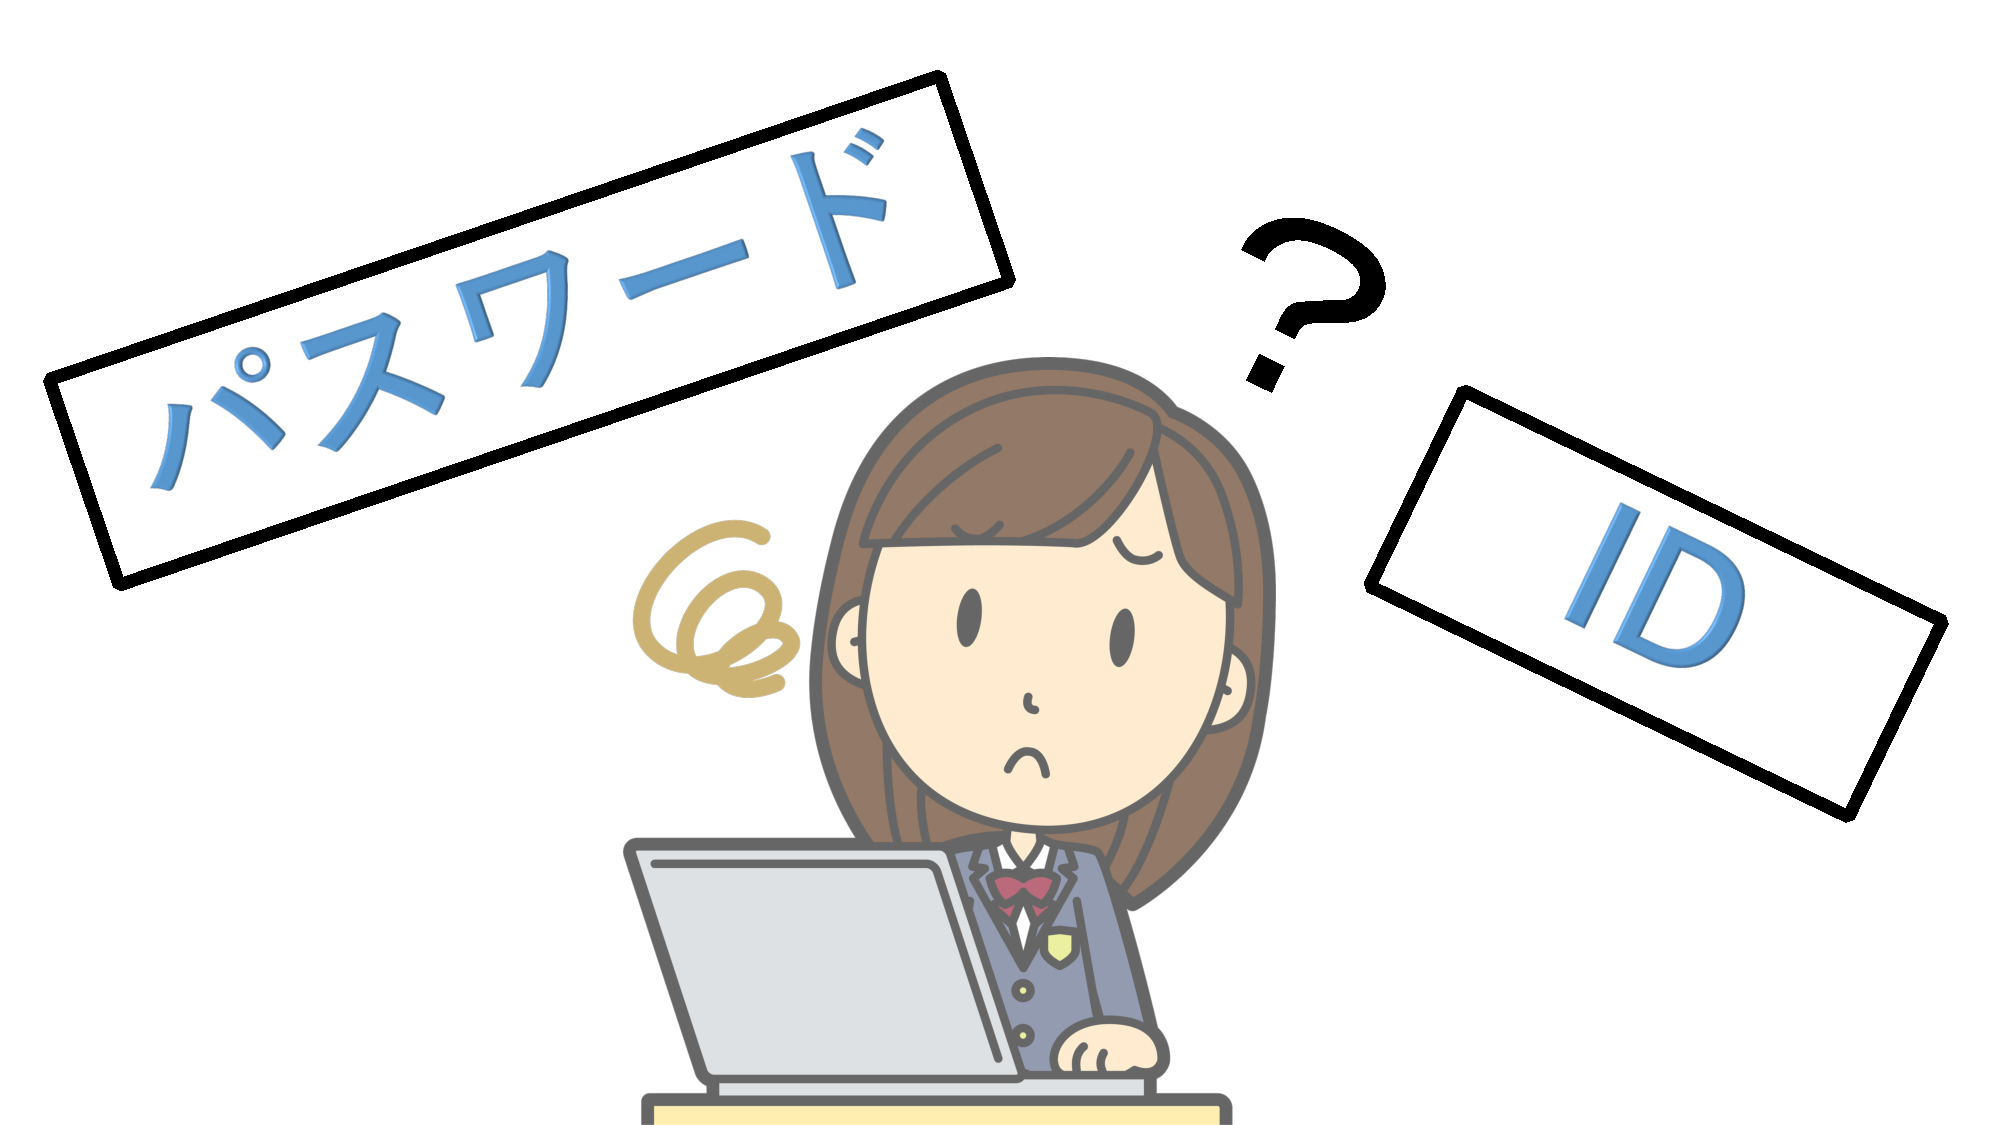
\includegraphics[width=70mm]{../../asset/image/fig_002_01_2025.pdf}
\end{figure}

IDやパスワードなど\ruby{認証}{にんしょう}で使っている\ruby{情報}{じょうほう}
（\ruby{身分証明書}{みぶんしょうめいしょ}）を\ruby{不適切}{ふてきせつ}な管理や、
\ruby{攻撃}{こうげき}などで\ruby{盗}{ぬす}まれてしまうと、なりすましなどの
\ruby{不正行為}{ふせいこうい}が行われてしまう\ruby{危険性}{きけんせい}もあります。
%
\begin{figure}[h]
  \centering
  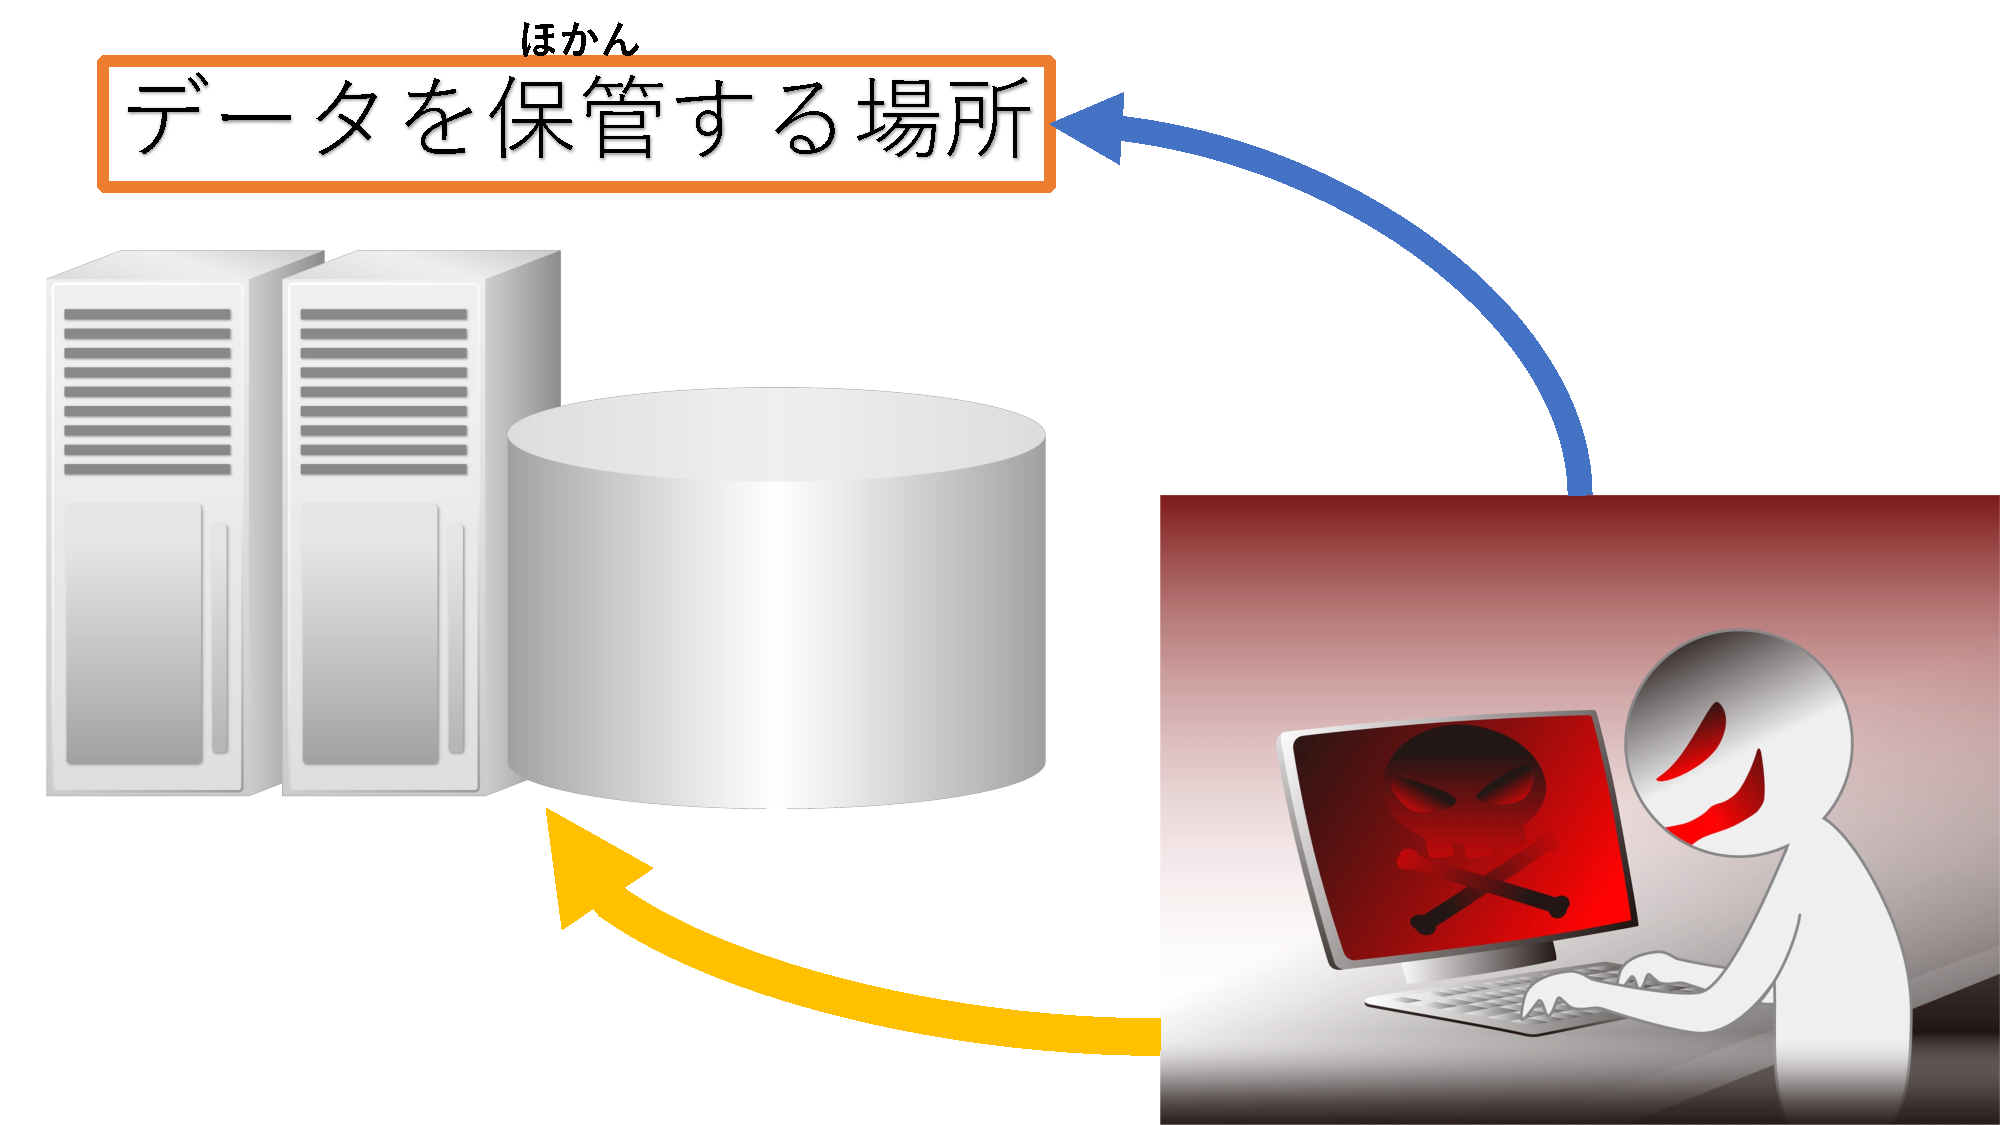
\includegraphics[width=70mm]{../../asset/image/fig_002_02_2025.pdf}
\end{figure}

このような手口による\ruby{被害}{ひがい}にあわないように、\ruby{認証}{にんしょう}の仕組みと
\ruby{重要性}{じゅうようせい}を\ruby{理解}{りかい}して、IDやパスワードを\ruby{厳重}{げんじゅう}に
管理しましょう。
%
\begin{figure}[h]
  \centering
  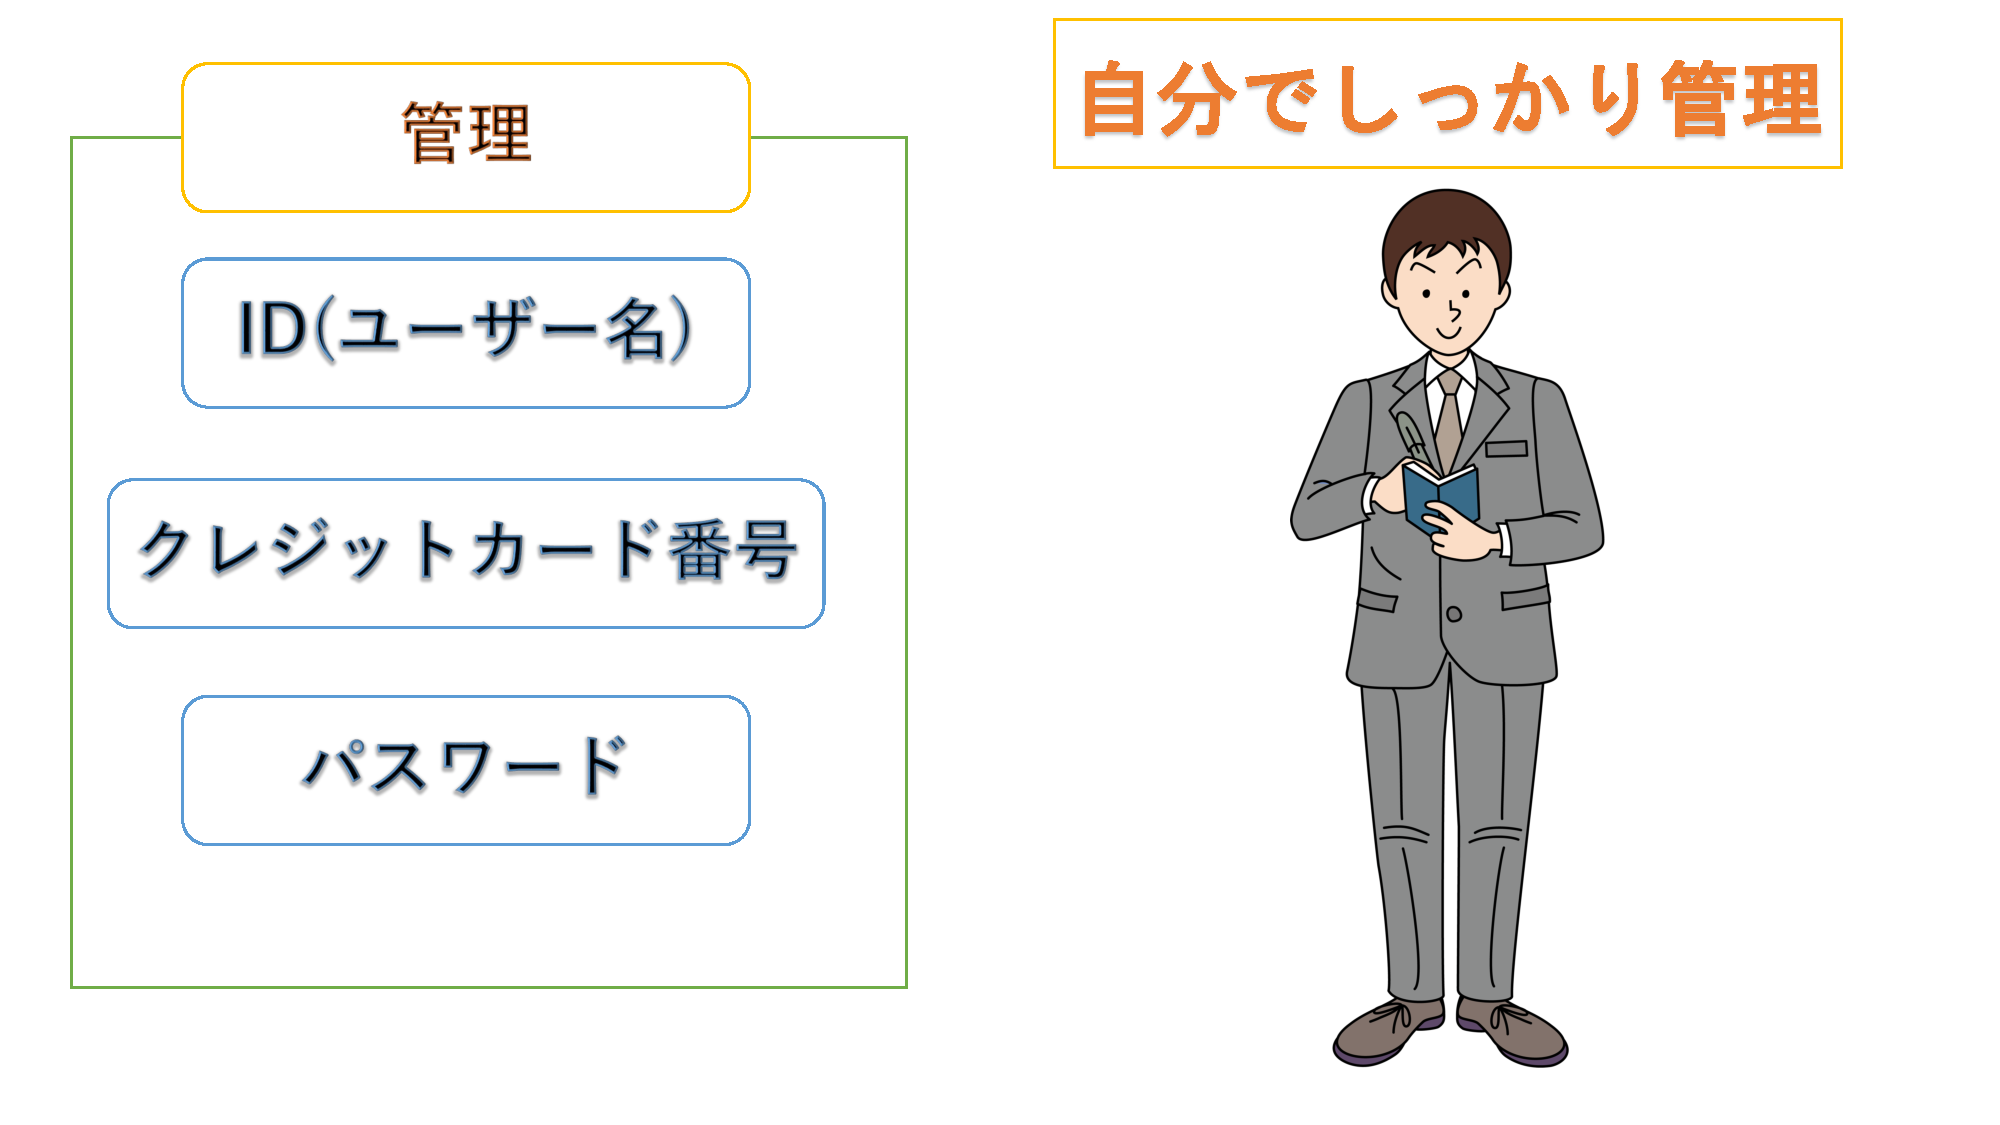
\includegraphics[width=70mm]{../../asset/image/fig_002_03_2025.pdf}
\end{figure}
\newpage

% 
% subsubsection
% 
\subsubsection{安全なパスワードの\ruby{設定}{せってい}や\ruby{適切}{適切}な管理について知ろう}
\footnote[0]{出典： \ruby{総務省}{そうむしょう}『国民のための\ruby{情報}{じょうほう}セキュリティサイト』
\url{https://www.soumu.go.jp/main_sosiki/joho_tsusin/security/basic/privacy/01-1.html}を加工して作成}

安全なパスワードとは他人に\ruby{推測}{すいそく}されにくく、計算で割り出しにくいものです。
そのためには、以下の点に注意することが大切です。
% \newline
 
\begin{itemize}
  \item 名前などの\ruby{個人情報}{こじんじょうほう}からは\ruby{推測}{すいそく}できないこと
  \item 英単語などをそのまま使用していないこと
  \item アルファベットと数字が\ruby{混在}{こんざい}していること
  \item \ruby{適切}{てきせつ}な長さの文字列であること
  \item \ruby{類推}{るいすい}しやすい\ruby{並}{なら}び方やその\ruby{安易}{あんい}な組合せにしないこと
\end{itemize}
%
\begin{figure}[h]
  \centering
  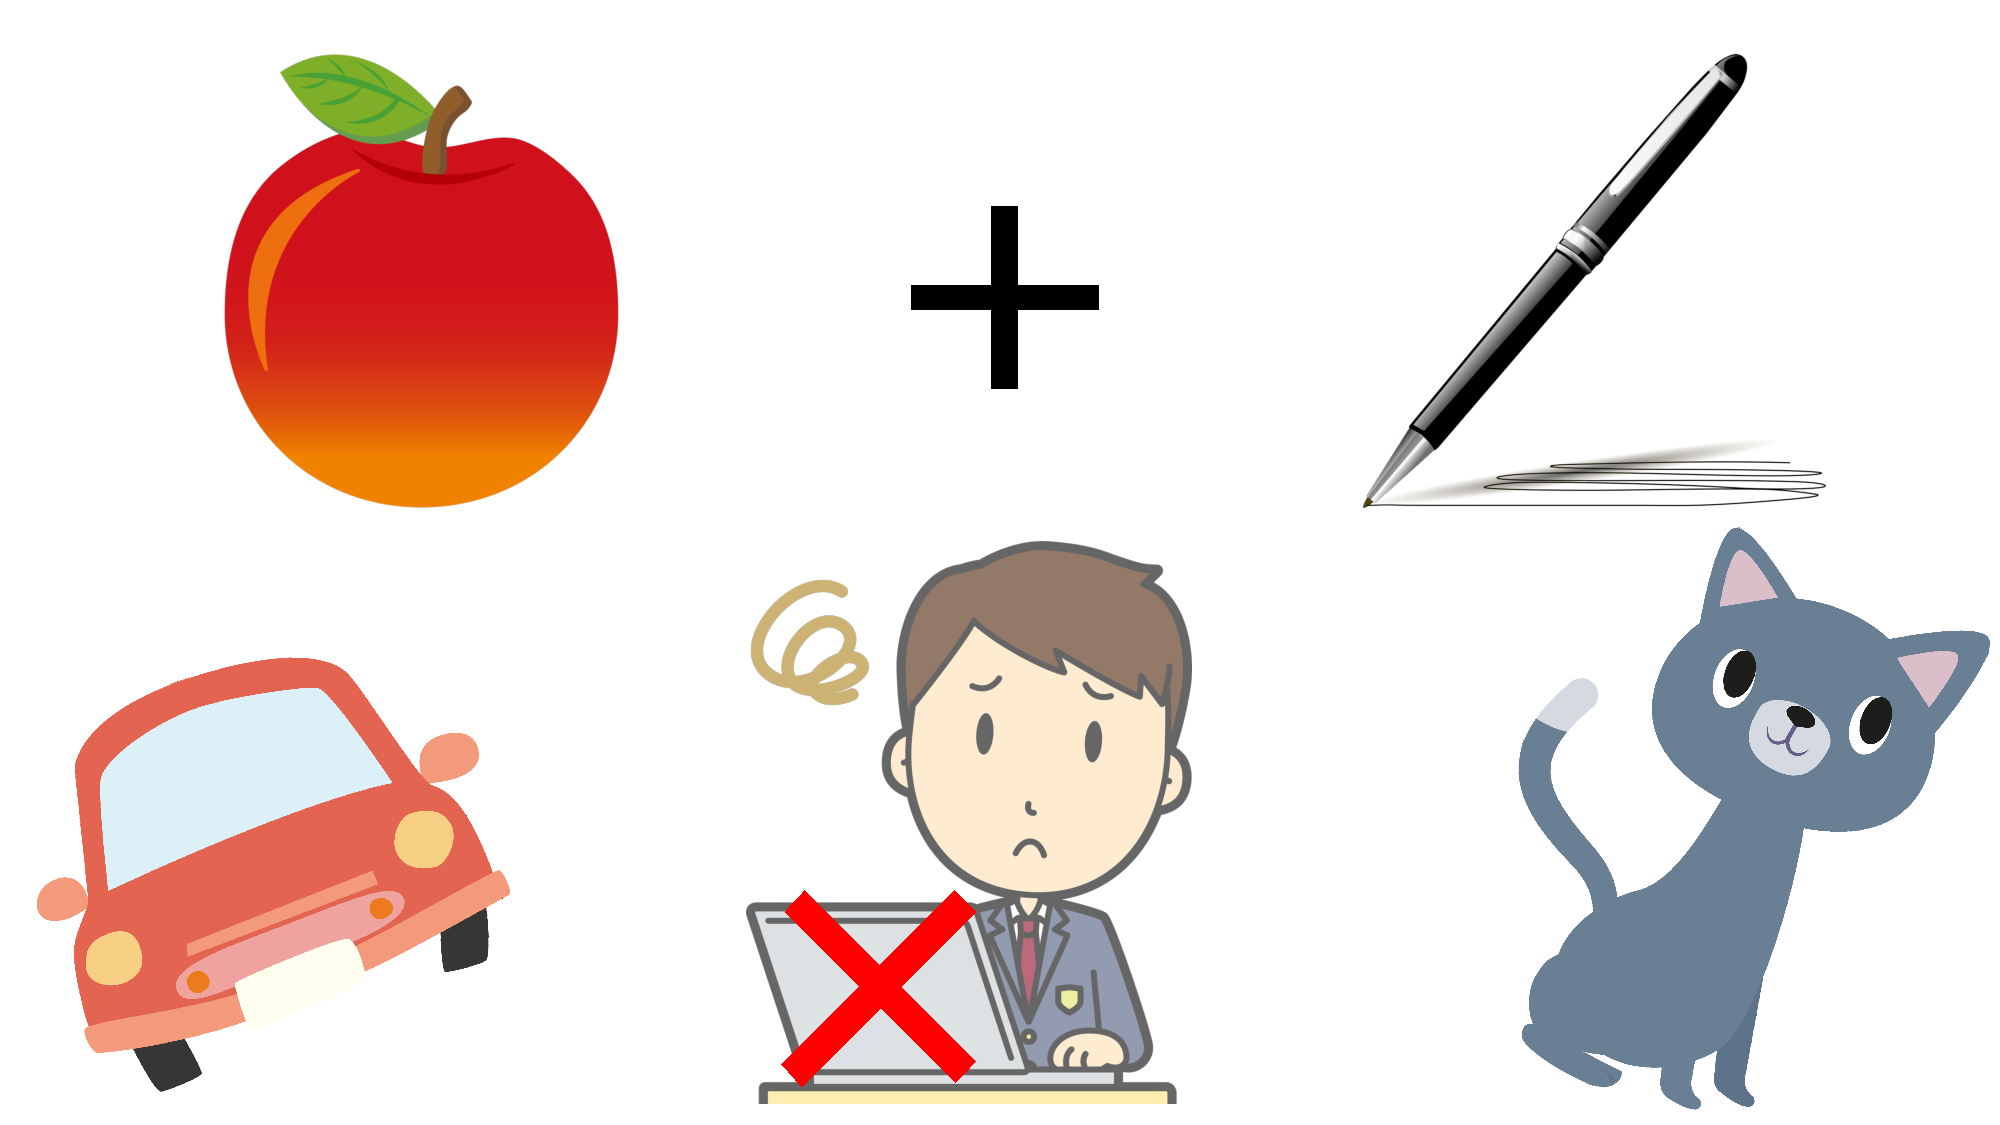
\includegraphics[width=70mm]{../../asset/image/fig_003_01_2025.pdf}
\end{figure}


パスワードはできる限り、\ruby{複数}{ふくすう}のサービスで使い回さないようにしましょう。
またパスワードを定期的に\ruby{変更}{へんこう}することを求められても、
\ruby{実際}{じっさい}にパスワードを\ruby{破}{やぶ}られアカウントが乗っ取られたり、
サービス側から流出した事実がなければパスワードを\ruby{変更}{へんこう}する必要はありません。
%
\begin{figure}[h]
  \centering
  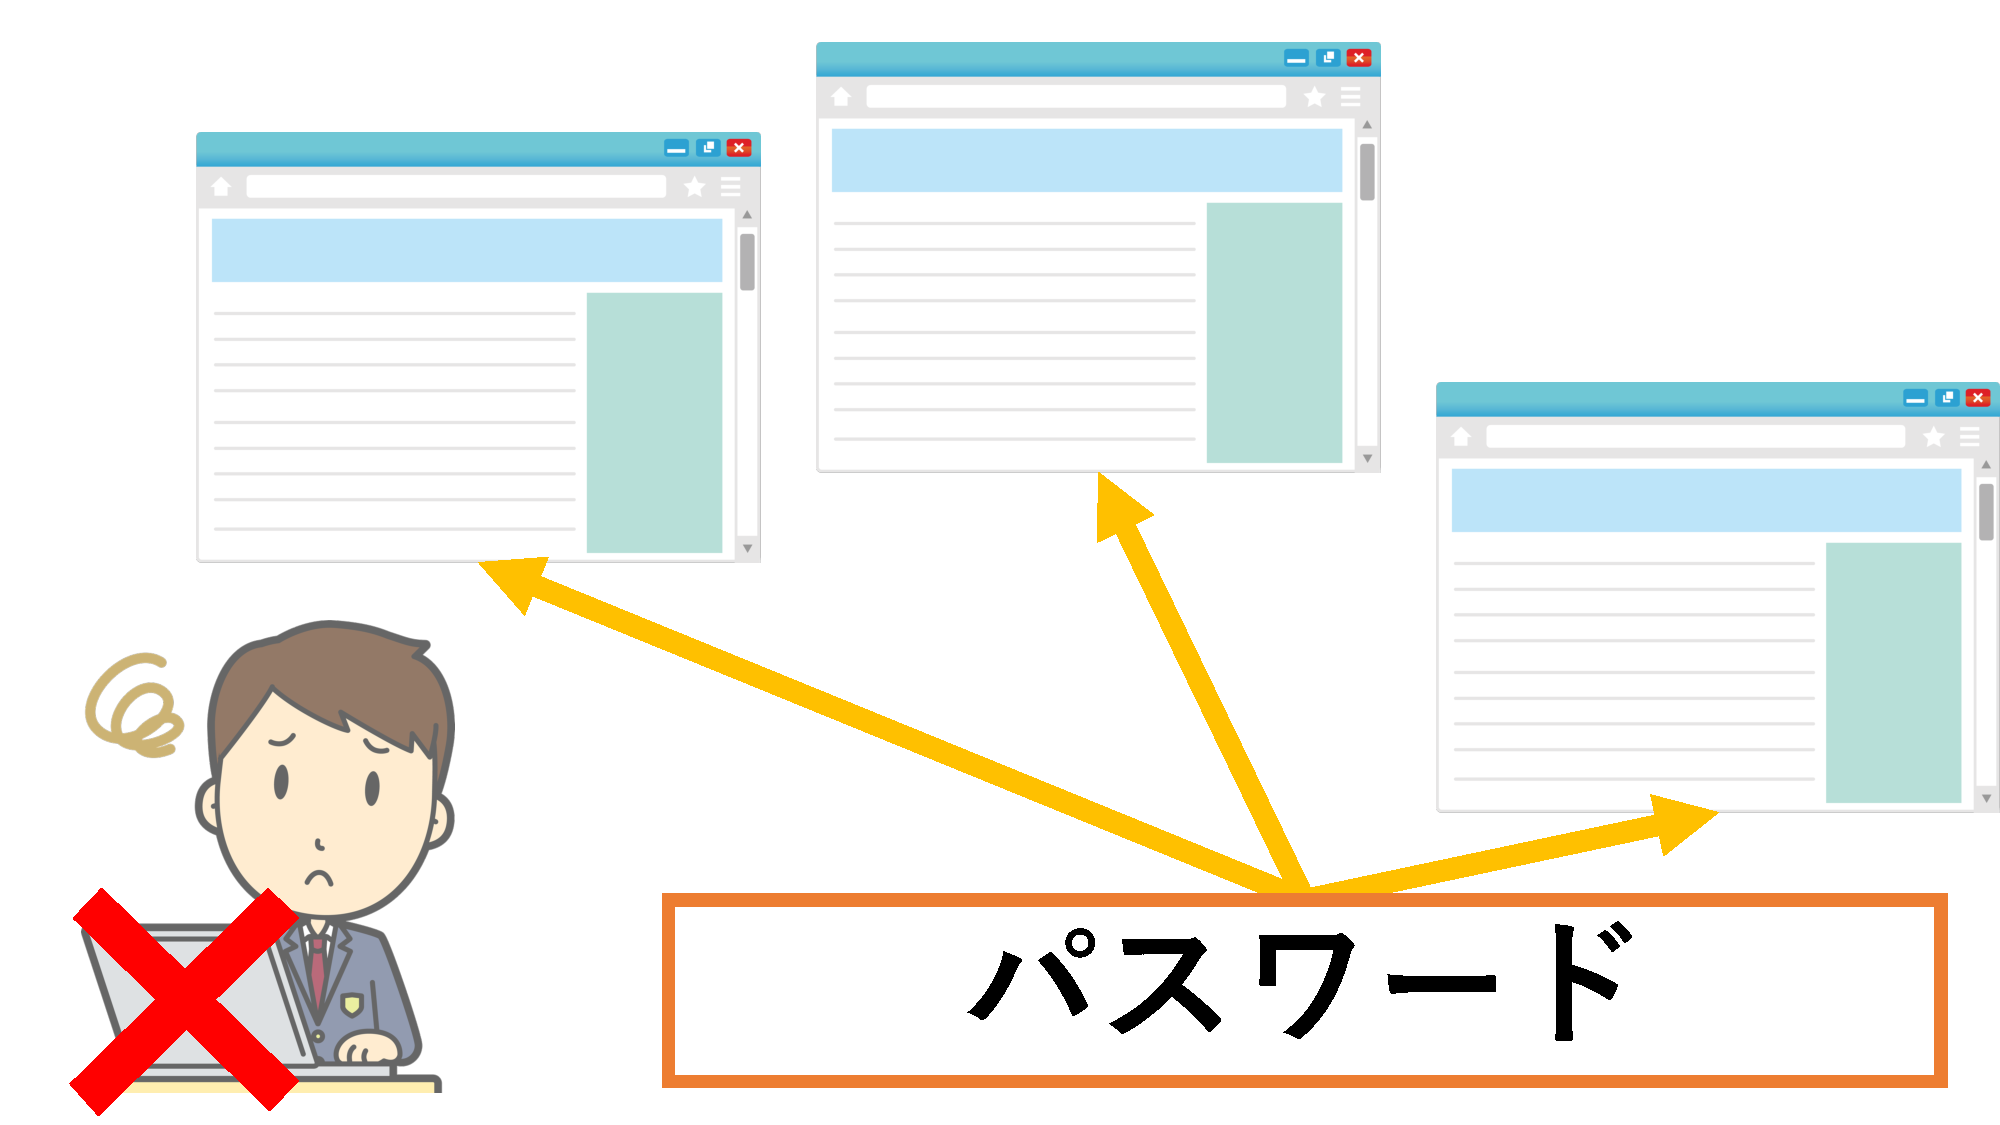
\includegraphics[width=70mm]{../../asset/image/fig_003_02_2025.pdf}
\end{figure}

安全なパスワードを\ruby{設定}{せってい}してもパスワードが他人に\ruby{漏}{も}れてしまえば
意味がありません。
以下に関して特に\ruby{留意}{りゅうい}が必要です。

\begin{itemize}
  \item パスワードは友人などに教えずに\ruby{秘密}{ひみつ}にすること
  \item パスワードをメールやSNSなどでやりとりしないこと
  \item パスワードのメモなどを他人の目に付く場所に\ruby{貼}{は}ったり置いたりしないこと
  \item パスワードをメモした場合は\ruby{鍵}{かぎ}のかかる\ruby{机}{つくえ}や金庫など安全に\ruby{保管}{ほかん}すること
\end{itemize}
\clearpage

% 
% subsubsection
% 
\subsubsection{パスワードの\ruby{制限}{せいげん}について知ろう}
\vspace*{5mm}

Linuxでは、ユーザー名とパスワードに関して、システムによって様々な\ruby{入力基準}{にゅうりょくきじゅん}が決められています。
パスワードについては、それぞれのシステムのパスワードポリシーと呼ばれる基準によって設定されています。
以下に、一般的な入力基準をあげます。

\begin{itemize}
  \item ユーザー名には小文字、数字、\verb|_|、のみ使用\ruby{可能}{かのう}
  \item ユーザー名の先頭に数字は使えない
  \item ユーザー名の長さは32文字以下（古いシステムでは8文字以下の場合もある）
  \item パスワードは8文字以上16文字以下
  \item パスワードには以下の4つのカテゴリタイプの文字をかならず入れる（大文字1文字以上、小文字1文字以上、数字1文字以上、英数字以外の文字1文字以上）
\end{itemize}


\begin{table}[htbp]
  \centering
  \caption{文字タイプ表}
  \begin{tabular}{|c|c|}
  \hline
      タイプ & \ruby{実際}{じっさい}に使用\ruby{可能}{かのう}な文字 \\
      \hline
      大文字& \verb|ABCDEFGHIJKLMNOPQRSTUVWXYZ| \\
      \hline
      小文字& \verb|abcdefghijklmnopqrstuvwxyz| \\
      \hline
      数字 & \verb|0123456789| \\
      \hline
      英数字以外の文字 & \verb|!@#$%^&*()_+`{}[]\:";'<>?,./| \textbar\\
      \hline
  \end{tabular}
\end{table}

\begin{itemize}
  \item \ruby{注意事項}{ちゅういじこう}
  \begin{itemize}
    % \item パスワードの先頭の大文字とパスワードの\ruby{末尾}{まつび}の数字は、使用される文字クラスの数にはカウントされません
    \item パスワードには辞書の単語やユーザーのログイン名を\ruby{含}{ふく}めることはできません
    \item 文字を数字または英数字以外の文字に置き\ruby{換}{か}えると、辞書の単語が受け入れられるようになります
  （例）\verb+app1e+, \verb+ta2ya+
    \item なるべく自分が覚えやすいものにしてください。
    ただし、\ruby{公}{おおやけ}になっている記号の\ruby{羅列}{られつ}やその他ですでに使用しているものは
    \ruby{避}{さ}けてください。 
  \end{itemize}
\end{itemize}
\clearpage



  \begin{tcolorbox}[title=\useOmetoi,breakable]
    自分のラズベリーパイのユーザ名とパスワードを考えましょう。
    \begin{enumerate}
      \addquiz{ユーザ名を決めて下の\ruby{記入欄}{きにゅうらん}に記入してみましょう。}
      \addquiz{パスワードを決めて下の\ruby{記入欄}{きにゅうらん}に記入してみましょう。}
    \end{enumerate}
  \end{tcolorbox}
  \vspace{10mm}
  \begin{tcolorbox}[title=\useOmetoi,breakable]
    次のパスワードに関する文章で正しいものには〇を、\ruby{誤}{あやま}っているものには×を記入してください。
    \begin{enumerate}
      \addox{名前などの\ruby{個人情報}{こじんじょうほう}から\ruby{推測}{すいそく}しやすい方が良い}
      \addox{英単語などをそのまま使用して良い}
      \addox{\ruby{適切}{てきせつ}な長さの文字列である方が良い}
      \addox{\ruby{類推}{るいすい}しやすい\ruby{並}{なら}び方やその\ruby{安易}{あんい}な組合せが良い}
      \addox{パスワードは友人などに教えずに\ruby{秘密}{ひみつ}にする}
      \addox{パスワードを送る時はメールやSNSなどで送る}
      \addox{パスワードをメモした場合は\ruby{鍵}{かぎ}のかかる\ruby{机}{つくえ}や金庫など安全な場所に\ruby{保管}{ほかん}する}
    \end{enumerate}
  \end{tcolorbox}
  \clearpage

  \begin{tcolorbox}[title=\useOmetoi,breakable]
    次はパスワードの例です。\ruby{安全性}{あんぜんせい}が高いパスワードには○を低いパスワードには×を記入してください。
    \begin{enumerate}
      \addox{Wp9jaFk6ag+koa0la\hspace{2mm}}
      \addox{Abcdefg123456789\hspace{6.5mm}}
      \addox{Or@ng3App13\hspace{14mm}}
      \addox{BananaPie2Me\hspace{13mm}}
    \end{enumerate}
  \end{tcolorbox}
\clearpage

% 
% subsection 1.1.11
% 
\subsection{ラズベリーパイを\ruby{準備}{じゅんび}しよう(手順)}

ラズベリーパイとマウス等を\ruby{接続}{せつぞく}して起動する\ruby{準備}{じゅんび}をします。

\begin{figure}[htbp]
  \centering
  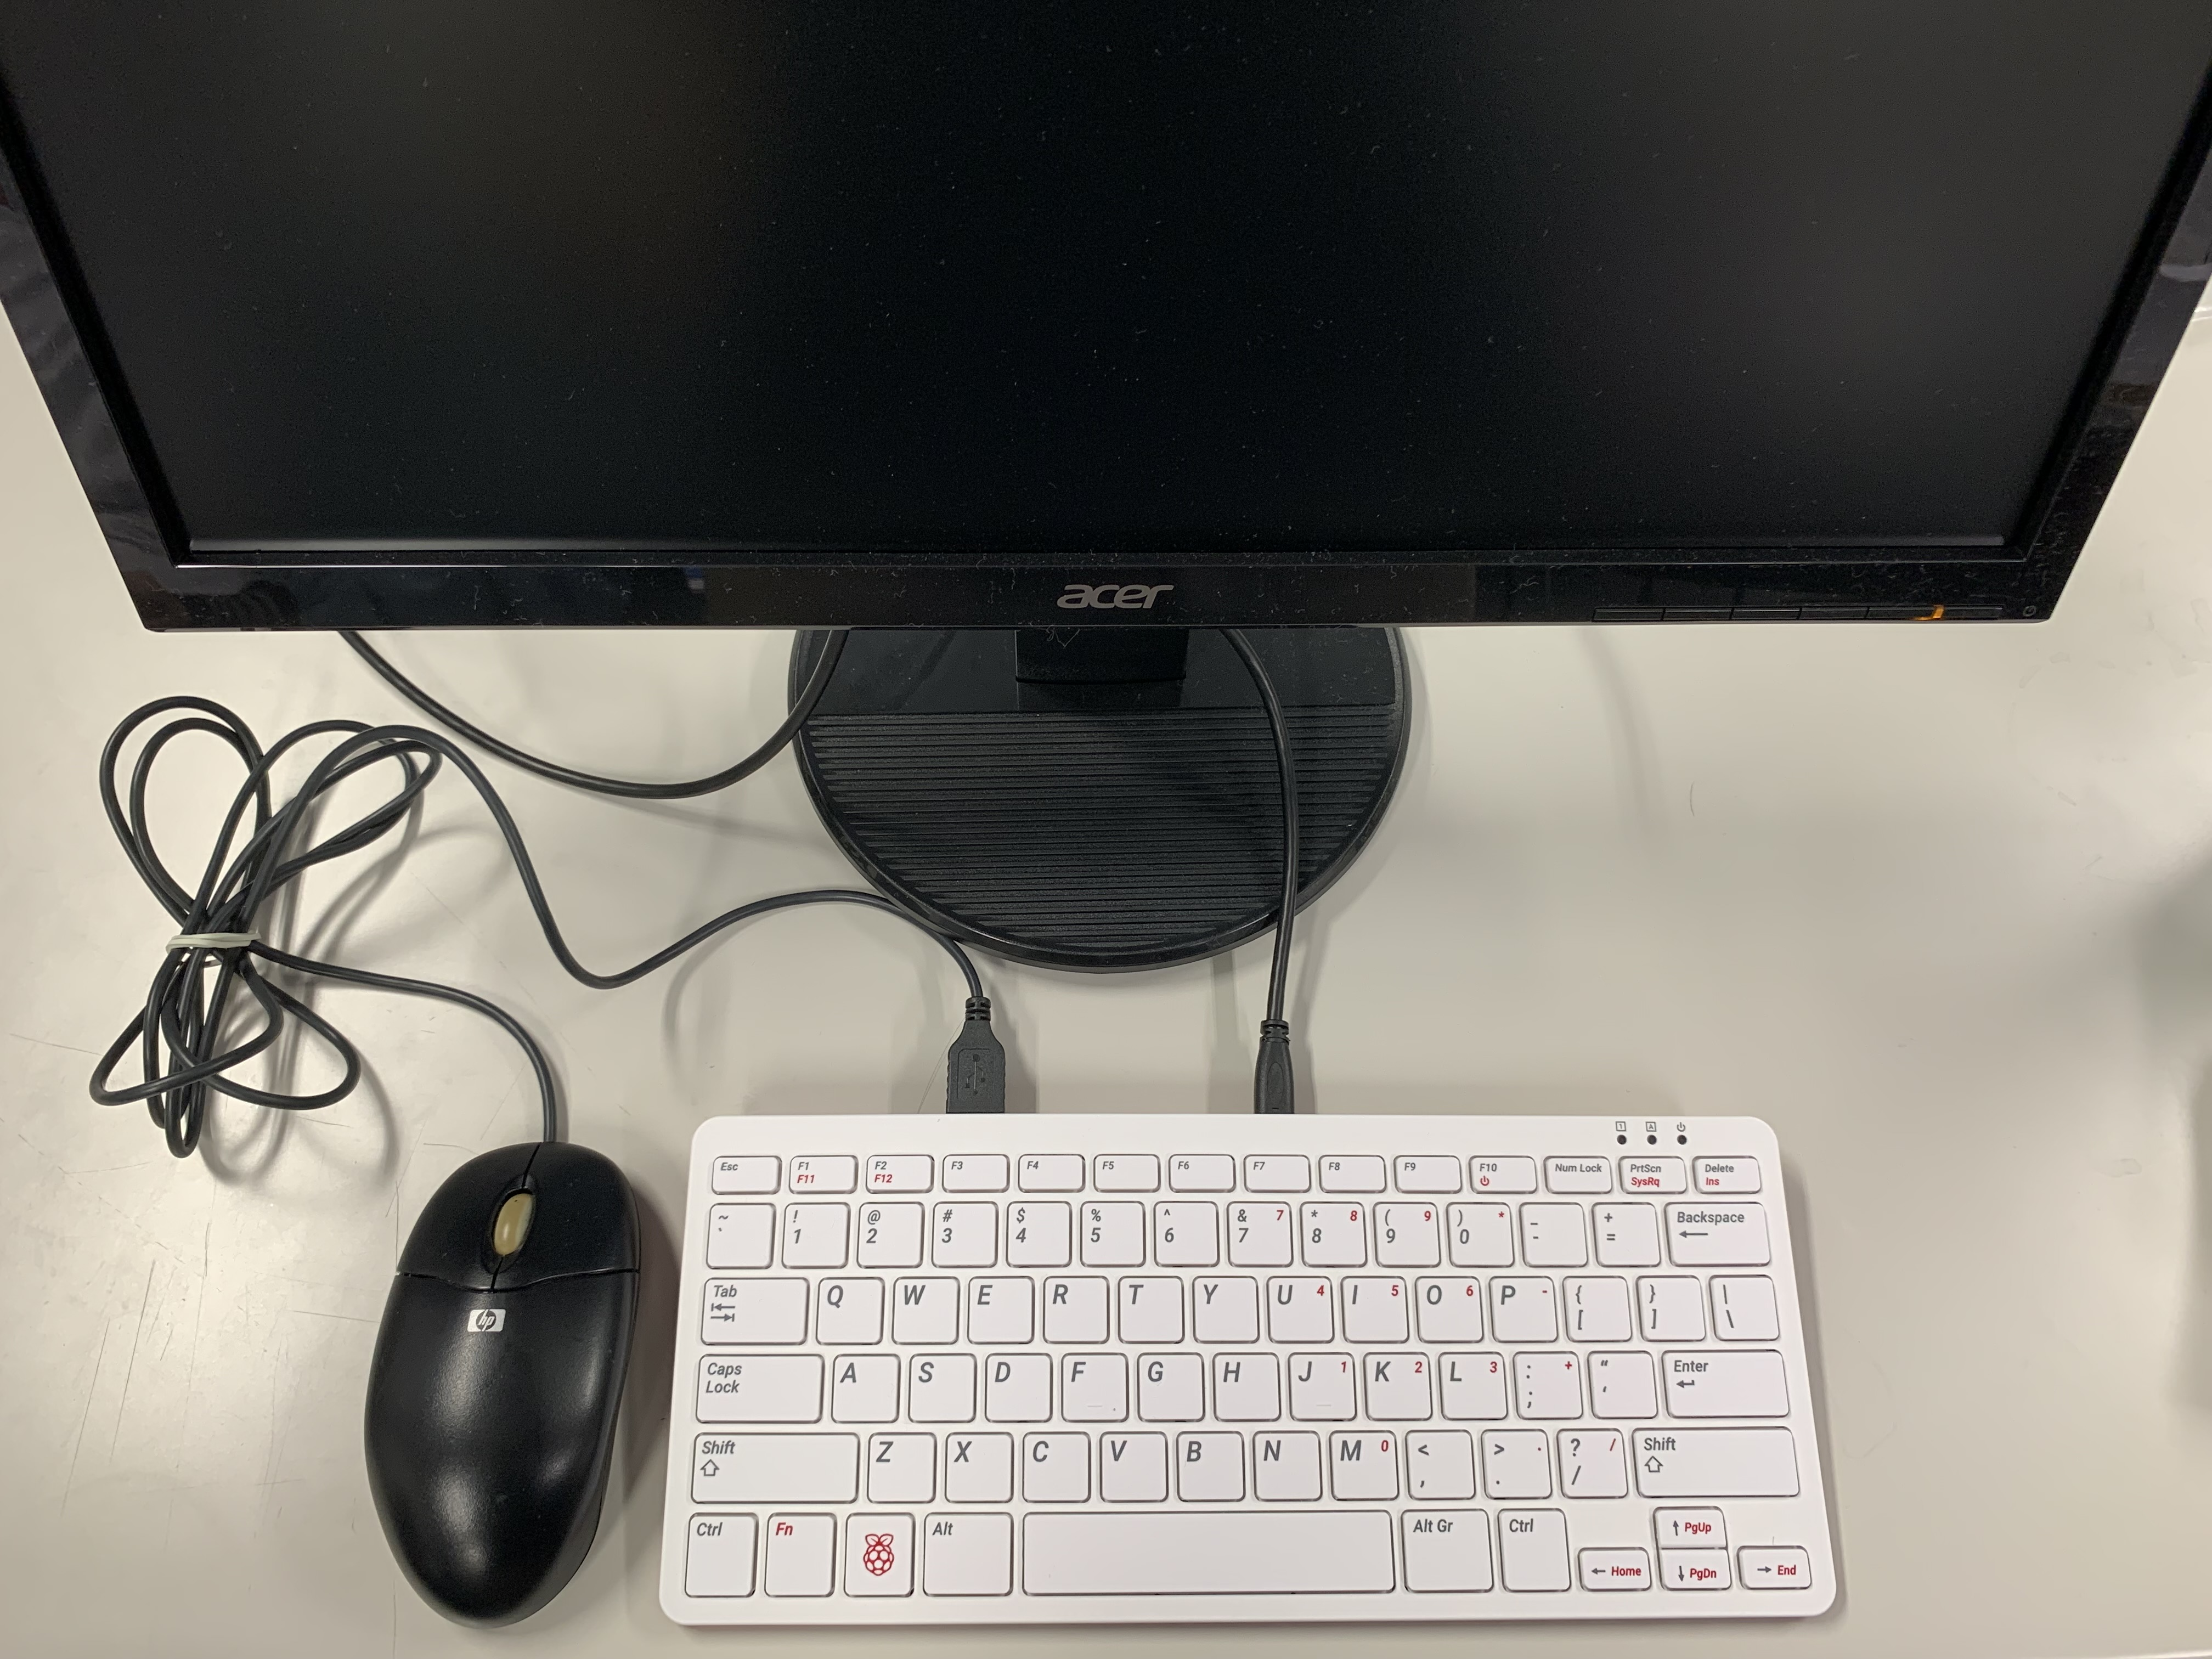
\includegraphics[keepaspectratio,height=60mm]{../../asset/image/connections01-2023.jpg}
  \caption{\ruby{接続}{せつぞく}の全体図}
  \label{fig:1}
\end{figure}

%
% subsubsection 1
%
\subsubsection{ラズベリーパイとモニタをつなぐ}

ラズベリーパイとモニタをHDMIケーブルで\ruby{接続}{せつぞく}します。
右側のHDMIポートを使用してください。
図~\ref{fig:2}、図~\ref{fig:3}を参考にしてください。
お家でやる場合は、モニタもしくはTVによってはHDMIの\ruby{差し込み}{さしこみ}口の場所が\ruby{異}{こと}なる場合があります。
%
\begin{figure}[htbp]
  \begin{minipage}[b]{0.6\linewidth}
    \centering
    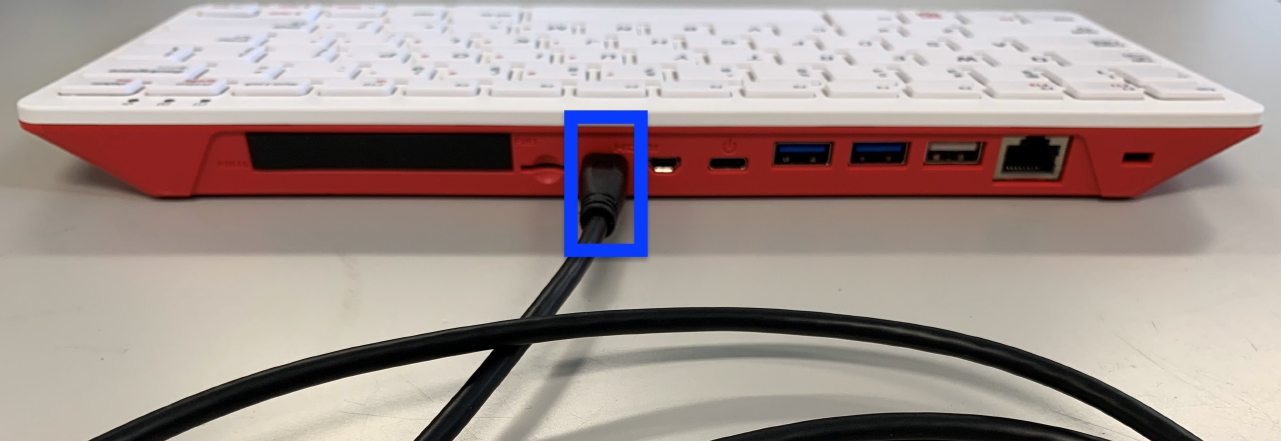
\includegraphics[keepaspectratio, height=30mm]{../../asset/image/figure22023.png}
    \caption{ラズベリーパイHDMI接続}
    \label{fig:2}
  \end{minipage}
  %
  \begin{minipage}[b]{0.35\linewidth}
    \centering
    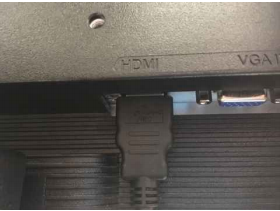
\includegraphics[keepaspectratio, height=30mm]{../../asset/image/textbook-img016.png}
    \caption{ディスプレイHDMI接続}
    \label{fig:3}
  \end{minipage}
\end{figure}
%

%
% subsubsection 2
%
\subsubsection{マウスをつなぐ}

マウスの先(USBコネクタ)をラズベリーパイへ差し\ruby{込}{こ}みます。
方向に注意してください。
%
\begin{figure}[htbp]
  \centering
  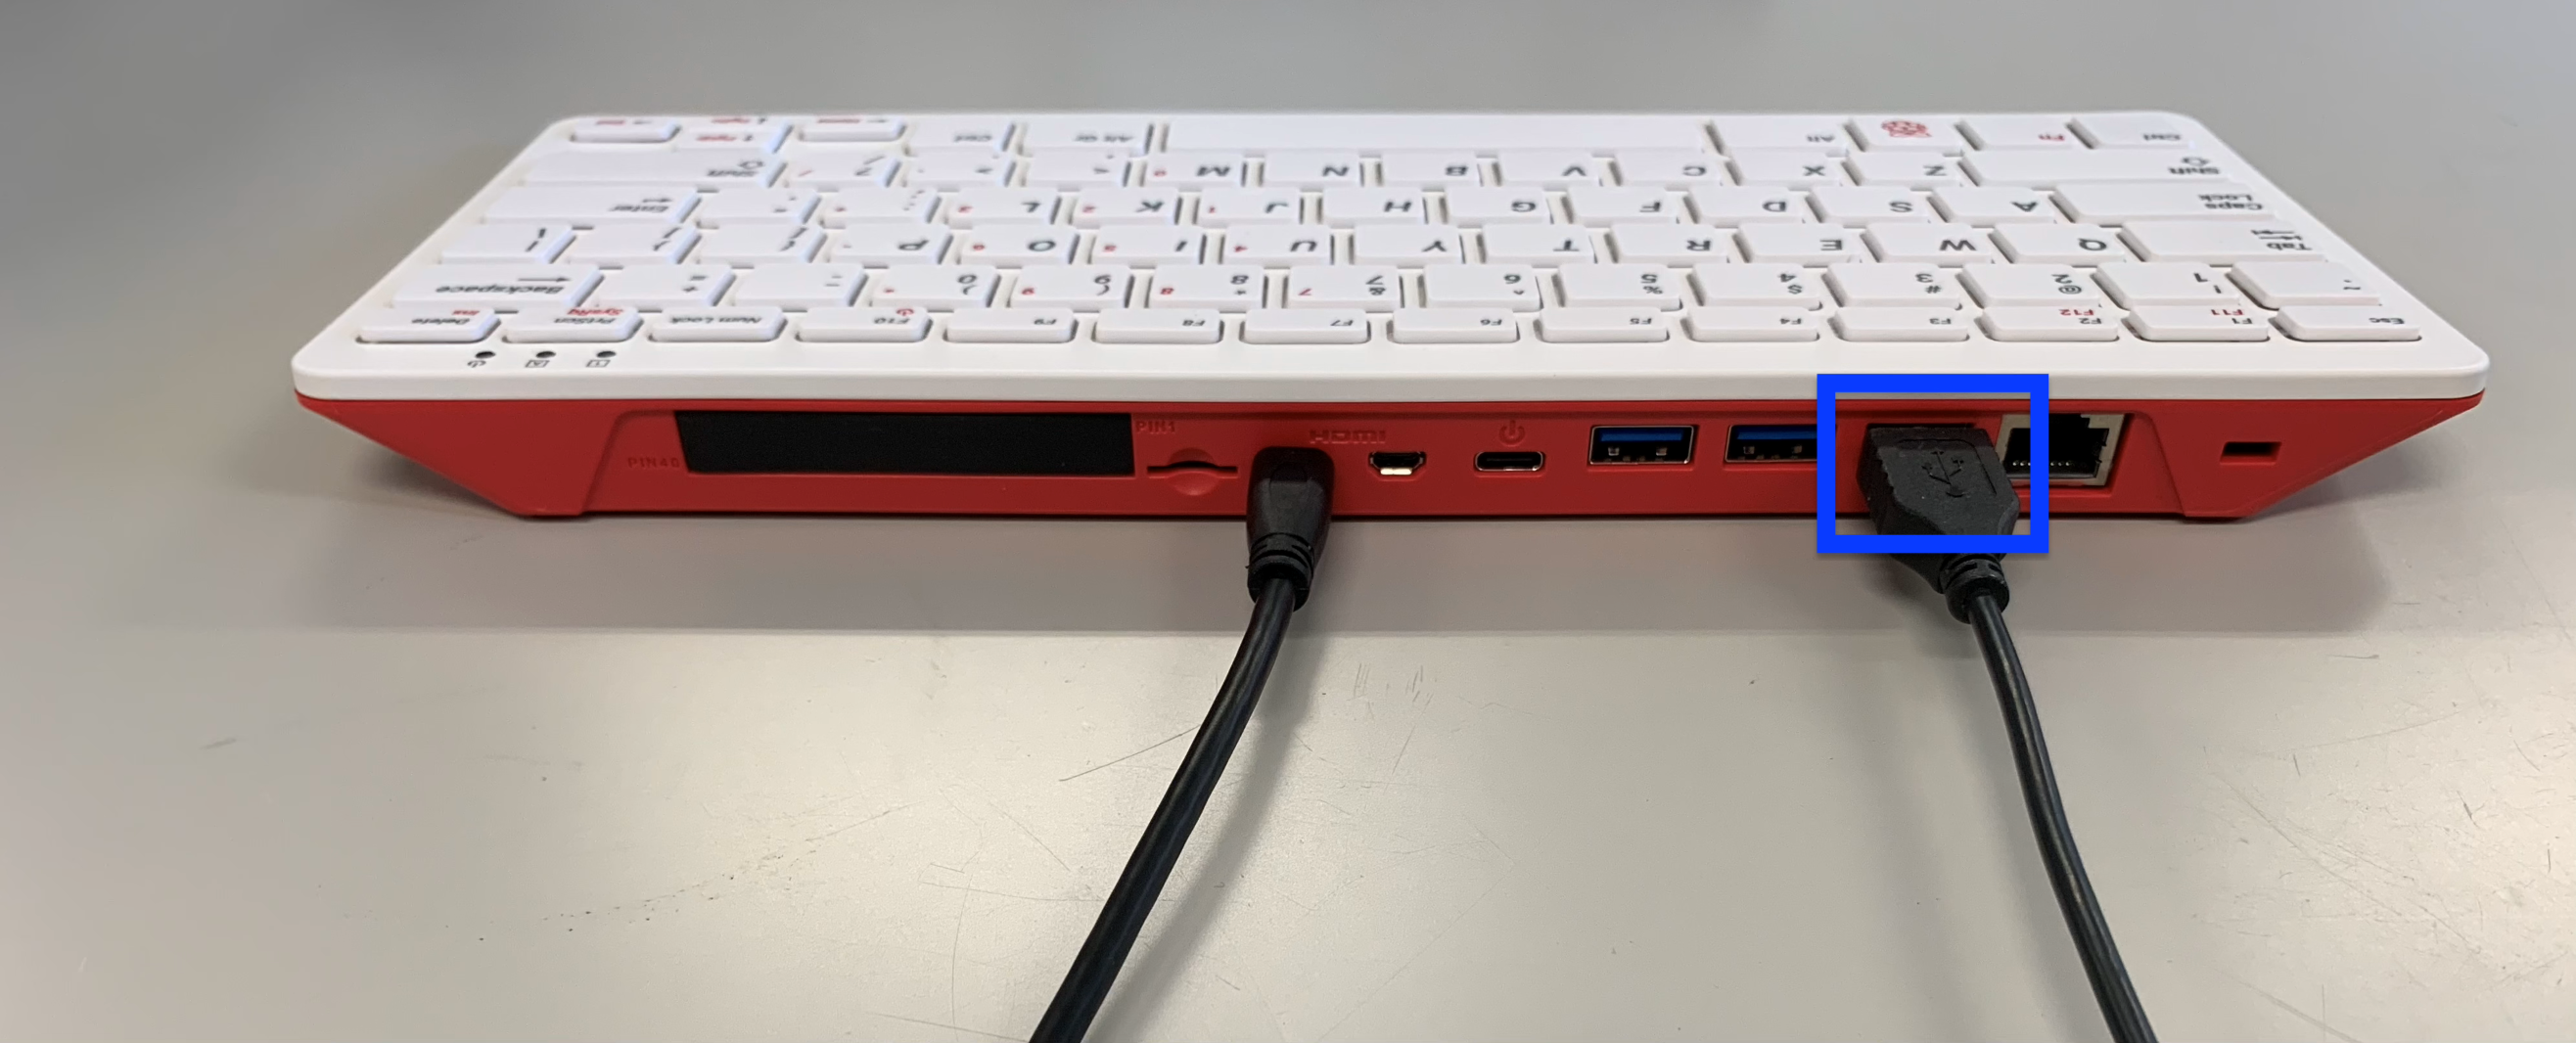
\includegraphics[keepaspectratio, height=30mm]{../../asset/image/figure1.10-4.png}
  \caption{マウスの\ruby{接続}{せつぞく}}
  \label{fig:4}
\end{figure}

%
% subsubsection 3
%
\subsubsection{microSD（マイクロエスディー）カードをいれる}

microSDカードをラズベリーパイ本体にさします。方向に注意してください。小さいのでなくさないように気をつけましょう。
%
\begin{figure}[htbp]
  \centering
  \includegraphics[keepaspectratio, height=30mm]{../../asset/image/figure1.10-5.png}
  \caption{microSDカードの差し\ruby{込}{こ}み}
  \label{fig:5}
\end{figure}

%
% subsubsection 4
%
\subsubsection{モニタの\ruby{電源}{でんげん}をいれる}

次にモニタのコンセントをさします。
モニタの右はじのボタンをおします。
電源が入ると青色にてんとうします。
お家でやるときは\ruby{電源}{でんげん}をいれた後に、入力きりかえが必要となる場合があります。
%
\begin{figure}[htbp]
  \centering
  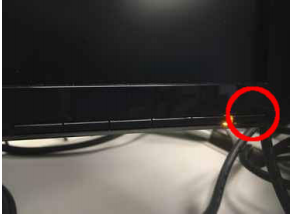
\includegraphics[keepaspectratio, height=30mm]{../../asset/image/textbook-img019.png}
  \caption{モニタの電源ボタンの位置}
  \label{fig:6}
\end{figure}

%
% subsubsection 5
%
\subsubsection{ラズベリーパイの\ruby{電源}{でんげん}をいれる}

最後にラズベリーパイの電源をいれます。
図~\ref{fig:7}のようにラズベリーパイに電源ケーブルをさしてコンセントへ\ruby{接続}{せつぞく}します。
緑色のランプがついてディスプレイにラズベリーが\ruby{表示}{ひょうじ}されます（図~\ref{fig:8}）。
%
\begin{figure}[htbp]
  \begin{minipage}[b]{0.5\linewidth}
    \centering
    \includegraphics[keepaspectratio, height=30mm]{../../asset/image/textbook-img020-2023.png}
    \caption{ラズベリーパイの電源\ruby{接続}{せつぞく}}
    \label{fig:7}
  \end{minipage}
  %
  \begin{minipage}[b]{0.5\linewidth}
    \centering
    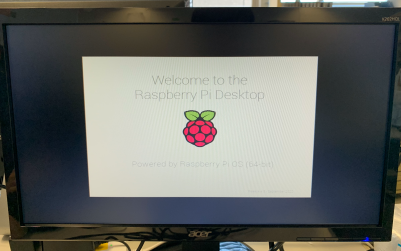
\includegraphics[keepaspectratio, height=30mm]{../../asset/image/textbook-img0212023.png}
    \caption{起動中の画面}
    \label{fig:8}
  \end{minipage}
\end{figure}
%
\clearpage


% 
% subsection
% 
\subsection{セットアップを始めよう}

% 
% subsubsection 1
% 
\subsubsection{言語とタイムゾーンの設定}

まずは定住国を\ruby{設定}{せってい}して、言語とタイムゾーンを決定します。
Raspberry pi 400 が起動すると、下の図~\ref{fig:9}のようなセットアップの開始画面になります。
この画面ではそのままNextボタンを\ruby{押}{お}して次に進みます。

\begin{figure}[htbp]
  \centering
  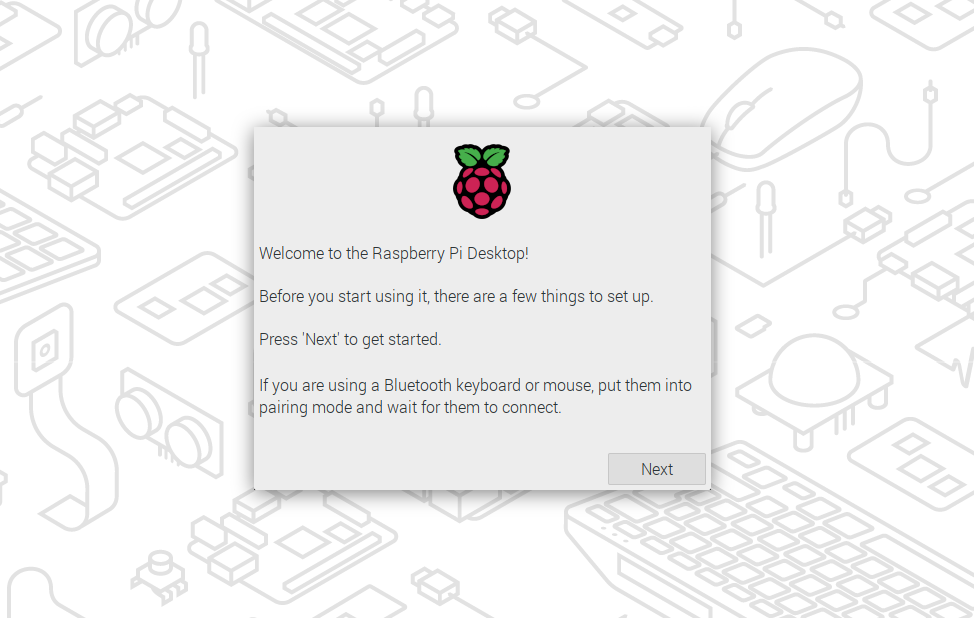
\includegraphics[keepaspectratio, height=50mm]{../../asset/image/sw_image01.png}
  \caption{起動後の画面}
  \label{fig:9}
\end{figure}

次の画面（図~\ref{fig:10}）で、自分の住んでいる国、言語、タイムゾーンを設定します。
\ruby{皆}{みな}さんは日本に住んでいますので、Countryの横のリストボタンをクリックして、
\ruby{候補}{こうほ}の中からJapanを選択します（図~\ref{fig:11}）。
Japanを選択すると、LanguageとTimezoneの\ruby{項目}{こうもく}が、自動的にそれぞれJapanese、Tokyoにかわります。
これらはそれぞれ使用する言語とタイムゾーンを表しています。
選択項目が、Japan、Japanese、Tokyoになっていることを確認してください。
次に、図~\ref{fig:10}中のピンクの\ruby{枠}{わく}の場所にチェックが入っていることを
\ruby{確認}{かくにん}して、Nextボタンを\ruby{押}{お}します。
%
\begin{figure}[htbp]
  \begin{minipage}[b]{0.5\linewidth}
    \centering
    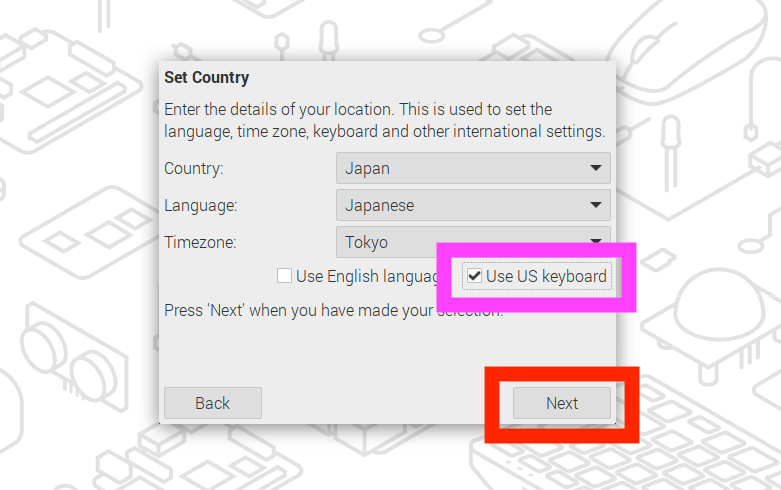
\includegraphics[keepaspectratio, height=50mm]{../../asset/image/sw_image02.png}
    \caption{国，言語，タイムゾーンの設定}
    \label{fig:10}
  \end{minipage}
  %
  \begin{minipage}[b]{0.5\linewidth}
    \centering
    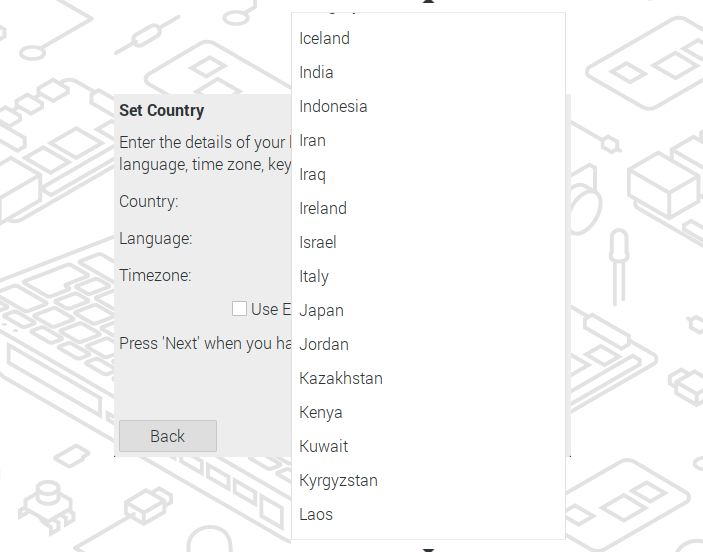
\includegraphics[keepaspectratio, height=50mm]{../../asset/image/sw_image03-2.png}
    \caption{Countryの\ruby{選択}{せんたく}}
    \label{fig:11}
\end{minipage}
\end{figure}
%
  

一般的に日本で使用されているキーボードの配列は、日本語配列（JIS配列）と呼ばれています。
\ruby{未来塾}{みらいじゅく}では、コンピュータの\ruby{専門家}{せんもんか}に多く使われている
米国のUS配列のキーボードを使用します。
キーの種類や\ruby{並}{なら}びは国や\ruby{規格}{きかく}、機械などによって\ruby{異}{こと}なるものが
ありますので注意してください。
\clearpage 

% 
% subsubsection 2
% 
\subsubsection{パスワードとユーザー名（ID）の設定}

次にユーザーを作成します。
図~\ref{fig:12}のように、上から順にユーザー名、パスワード、パスワード（再入力）用のテキストボックスが表示されます。
  
\begin{figure}[h]
  \centering
  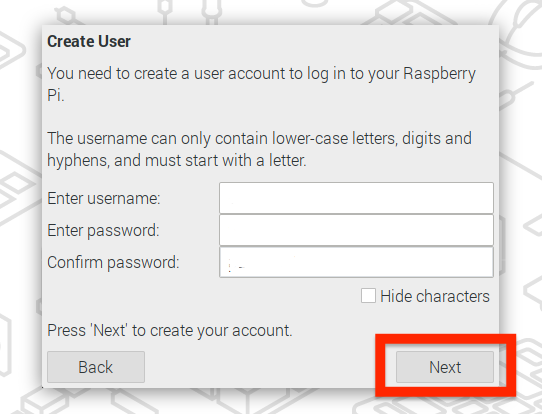
\includegraphics[keepaspectratio, height=45mm]{../../asset/image/sw_image03.png}
  \caption{ユーザーの作成}
  \label{fig:12}
\end{figure}

ここで、先ほどの問題1-1で記入したユーザー名とパスワードを\ruby{実際}{じっさい}に入力します。
その\ruby{際}{さい}に、下のような画面（図~\ref{fig:13}）が出てくることがあります。
このメッセージは、ユーザー名（ID）かパスワードのどちらかに不正な文字などが\ruby{含}{ふく}まれている
\ruby{可能性}{かのうせい}がある場合に表示されますので、
正しく入力できているか、もう一度\ruby{確認}{かくにん}しましょう。
  
\begin{figure}[h]
  \centering
  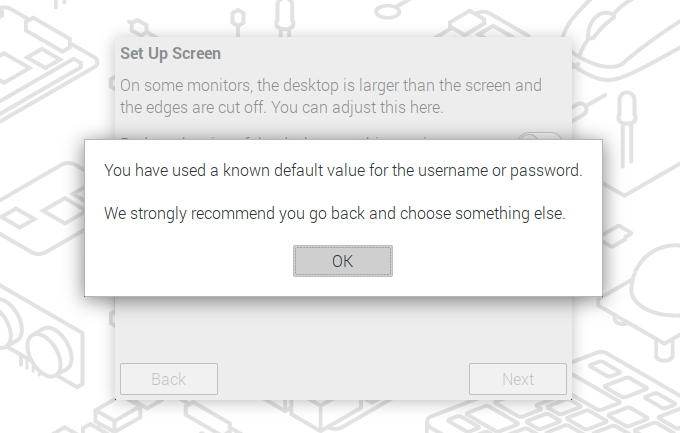
\includegraphics[keepaspectratio, height=45mm]{../../asset/image/sw_image04.png}
  \caption{エラー画面}
  \label{fig:13}
\end{figure}

ここで、画面が\ruby{歪}{ゆが}んだりしていないか、\ruby{縦横}{たてよこ}に\ruby{伸}{の}びていないかを
TAと\ruby{一緒}{いっしょ}に\ruby{確認}{かくにん}してください。
問題がない場合は、Nextボタンを\ruby{押}{お}して次に進みます。
% \clearpage


% 
%     \begin{figure}[h]
%     \centering
%     \begin{minipage}{5.228cm}
%       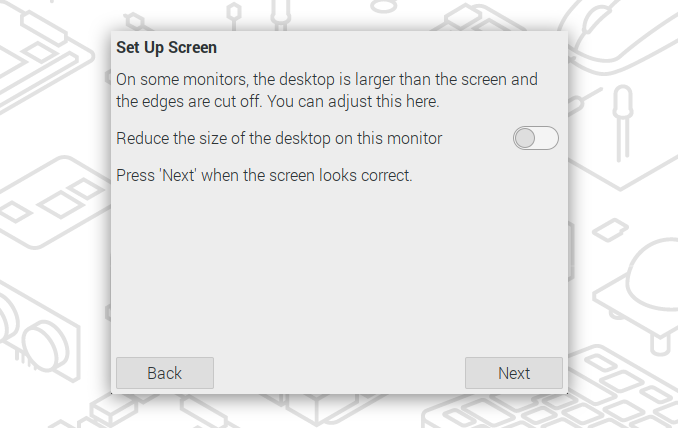
\includegraphics[width=6.000cm]{../../asset/image/sw_image05.png}
%       \caption{スクリーンサイズ\ruby{確認}{かくにん}}\label{fig:14}
%     \end{minipage}
%   \end{figure}
% 
\begin{figure}[h]
  \centering
  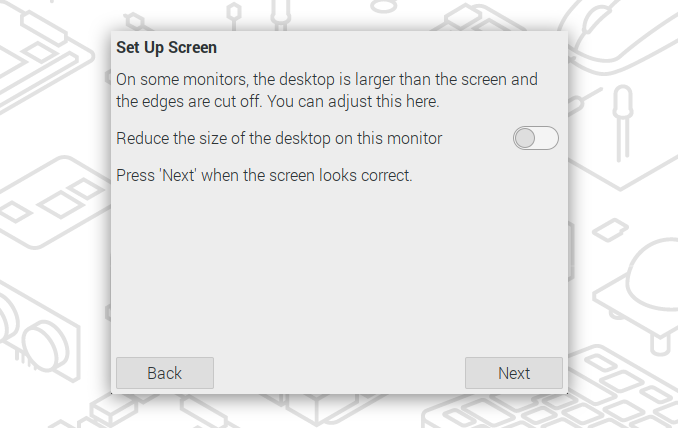
\includegraphics[keepaspectratio, height=45mm]{../../asset/image/sw_image05.png}
  \caption{スクリーンサイズの\ruby{確認}{かくにん}}
  \label{fig:14}
\end{figure}

% \clearpage



% 
% subsubsection 3
% 
\subsubsection{Wi-Fiに\ruby{接続}{せつぞく}する}

次にWi-Fiの\ruby{設定}{せってい}を行います。図~\ref{fig:15}の\ruby{赤枠}{あかわく}の中に
\ruby{接続可能}{せつぞくかのう}なWi-Fiの名前が\ruby{表示}{ひょうじ}されます。

\vspace*{10mm}

\begin{tcolorbox}[title=\useOmetoi,breakable]
  ここでは、使用するWi-Fiのアドレスとパスワードが必要となります。
  TAからアドレスとパスワードを教えてもらい、下の\ruby{欄}{らん}に記入しましょう。
  \begin{enumerate}
    \addquiz{Wi-Fiアドレスを\ruby{記入欄}{きにゅうらん}に記入しましょう。}
    \addquiz{Wi-Fiのパスワードを\ruby{記入欄}{きにゅうらん}に記入しましょう。}
  \end{enumerate}
\end{tcolorbox}

\vspace*{5mm}

上の問題で記入したWi-Fiのアドレスを\ruby{選択}{せんたく}して、Nextボタンを\ruby{押}{お}します。

\begin{figure}[H]
  \centering
  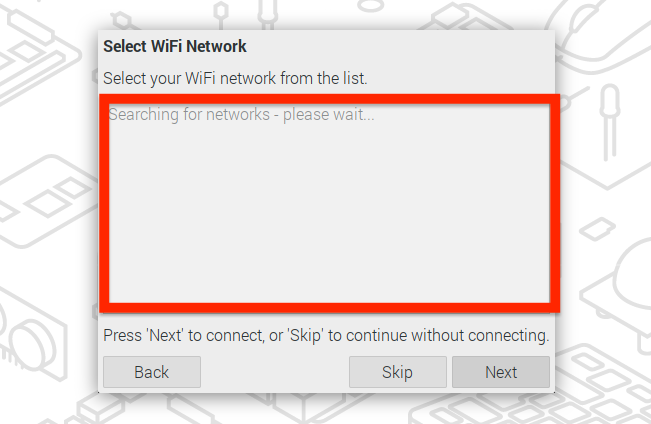
\includegraphics[keepaspectratio, height=50mm]{../../asset/image/sw_image06kai.png}
  \caption{Wi-Fiの\ruby{選択}{せんたく}}
  \label{fig:15}
\end{figure}

% 次にパスワードを入力するように求められますので、
\noindent%
次に、上の問題で記入したパスワードを入力してNextボタンを\ruby{押}{お}します。
\begin{figure}[H]
  \centering
  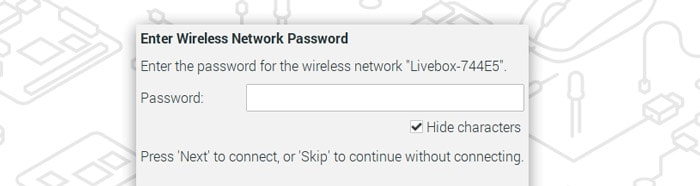
\includegraphics[keepaspectratio, height=25mm]{../../asset/image/rp_enter_wifi_password.jpg}
  \caption{Wi-Fiパスワードの入力}
  \label{fig:16}
\end{figure}
% \clearpage


% \subsection{ブラウザを選択しよう}

% 
% subsubsection 4
% 
\subsubsection{アップデートをスキップしてraspberry piを始めよう}

% 
% まず、デフォルトのブラウザを選択します。
% ここでは図~\ref{fig:16}の赤い枠のFirefoxを\ruby{選択}{せんたく}して、Nextボタンを\ruby{押}{お}します。

% \begin{figure}[H]
%   \centering
%   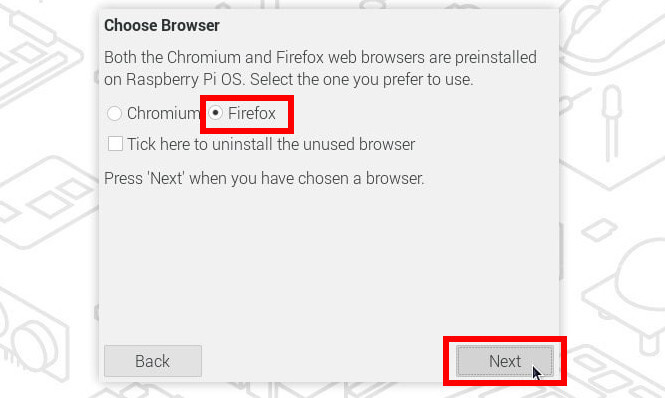
\includegraphics[keepaspectratio, height=50mm]{../../asset/image/2024_image01.jpg}
%   \caption{ブラウザの選択}
%   \label{fig:16}
% \end{figure}
% 

次の画面に進むと、ソフトウェアアップデートを求められますが、
\textbf{今回はアップデートをしないでください。図~\ref{fig:17}の}\textbf{\color{red}赤い枠のSkipボタン}を
\ruby{押}{お}して次の画面に進みます。

\begin{figure}[H]
  \centering
  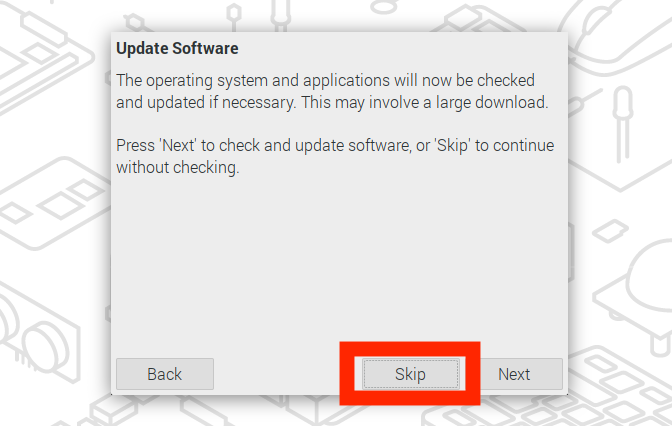
\includegraphics[keepaspectratio, height=50mm]{../../asset/image/sw_image07.png}
  \caption{ソフトウェアアップデート}
  \label{fig:17}
\end{figure}
% \clearpage

\noindent%
ここでアップデートしてしまうと、\ruby{授業}{じゅぎょう}で使う教材の一部が正しく動かなくなってしまいます。
もし、\ruby{間違}{まちが}えてアップデートをしてしまった場合には、
SDカードを\ruby{交換}{こうかん}する必要がありますので、すぐにTAに\ruby{相談}{そうだん}してください。\\
% \clearpage

これで、大まかな初期\ruby{設定}{せってい}が\ruby{完了}{かんりょう}しましたので、
ラズベリーパイを\ruby{再起動}{さいきどう}します。
画面右下にあるRestartボタンを\ruby{押}{お}してください。

\begin{figure}[H]
  \centering
  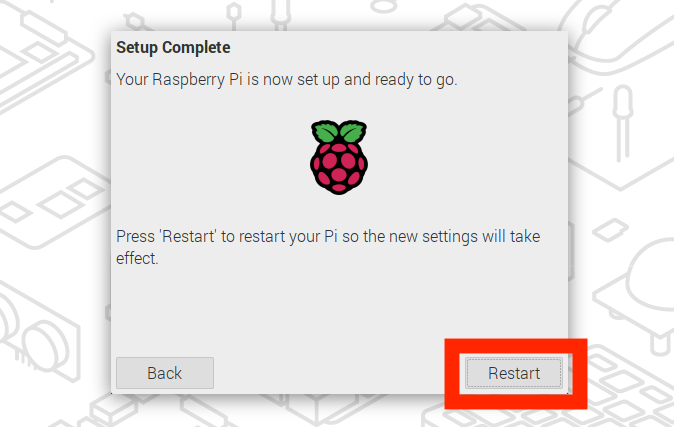
\includegraphics[keepaspectratio, height=50mm]{../../asset/image/sw_image08.png}
  \caption{\ruby{再起動}{さいきどう} }
  \label{fig:18}
\end{figure}

\clearpage

\end{document}
